\documentclass{beamer}
\usepackage[utf8]{inputenc}
\usepackage{amsmath, amssymb, bm}
\usepackage{physics}
\usepackage{graphicx}
\usepackage{hyperref}
\usepackage{xmpmulti}
\usepackage{tikz}
\usetheme{Madrid} % You can change the theme as you like
\usecolortheme{seagull}


\begin{document}

\title[Quantum Computing and ML]{\textbf{Quantum Computing, why should we think of that?}}
\author{Nuclear TALENT course on Quantum Computing for Nuclear Physics}
\institute{European Center for Theoretical Nuclear Physics and Related Areas, Trento, Italy}
\date{Monday June 16, 2025}
\maketitle

%-----------------------------------------------------------
%\begin{frame}
%    \titlepage
%\end{frame}

%-----------------------------------------------------------





%-----------------------------------------------------------
\section{Introduction to Quantum Computing}
\begin{frame}{What is Quantum Computing?}
Quantum computing leverages principles of quantum mechanics to perform computations beyond classical capabilities.

\vspace{10pt}
\textbf{Key Concepts:}
\begin{itemize}
\item \textbf{Superposition:} Qubits can exist in a combination of states.
\item \textbf{Entanglement:} Correlation between qubits regardless of distance.
\item \textbf{Quantum Interference:} Probability amplitudes interfere to solve problems.
\end{itemize}

\textbf{Qubit Representation:}
\[
\ket{\psi} = \alpha \ket{0} + \beta \ket{1}, \quad |\alpha|^2 + |\beta|^2 = 1
\]
\end{frame}


%-----------------------------------------------------------
\section{Quantum Machine Learning (QML)}
\begin{frame}{What is Quantum Machine Learning?}
\textbf{Quantum Machine Learning (QML)} integrates quantum computing with machine learning algorithms to exploit quantum advantages.

\vspace{10pt}
\textbf{Motivation:}
\begin{itemize}
    \item High-dimensional Hilbert spaces for better feature representation.
    \item Quantum parallelism for faster computation.
    \item Quantum entanglement for richer data encoding.
\end{itemize}


\end{frame}

\section{Quantum Speedups}
\begin{frame}{Quantum Speedups}
\textbf{Why Quantum?}
\begin{itemize}
    \item \textbf{Quantum Parallelism:} Process multiple states simultaneously.
    \item \textbf{Quantum Entanglement:} Correlated states for richer information.
    \item \textbf{Quantum Interference:} Constructive and destructive interference to enhance solutions.
\end{itemize}

\textbf{Example - Grover's Algorithm:}
\[
\text{Quantum Search Complexity: } O(\sqrt{N}) \text{ vs. } O(N)
\]

\textbf{Advantage:}
- Speedups in high-dimensional optimization and linear algebra problems.
\end{frame}

%-----------------------------------------------------------
\section{Challenges in Quantum Technology}
\begin{frame}{Challenges and Limitations}
\textbf{1. Quantum Hardware Limitations:}
\begin{itemize}
    \item Noisy Intermediate-Scale Quantum (NISQ) devices.
    \item Decoherence and limited qubit coherence times.
\end{itemize}

\textbf{2. Data Encoding for QML:}
\begin{itemize}
    \item Efficient embedding of classical data into quantum states.
\end{itemize}

\textbf{3. Scalability:}
\begin{itemize}
    \item Difficult to scale circuits to large datasets.
\end{itemize}
\end{frame}




\begin{frame}{What is Quantum Entanglement?}
\textbf{Quantum Entanglement} is a quantum phenomenon where two or more particles become correlated in such a way that the state of one particle directly affects the state of the other, regardless of distance.

\vspace{10pt}
\textbf{Key Features:}
\begin{itemize}
    \item Non-local correlations
    \item No classical analog
    \item Violates Bell's inequalities
\end{itemize}

\textbf{Entangled State Example:}
\[
\ket{\Phi^+} = \frac{1}{\sqrt{2}} (\ket{00} + \ket{11})
\]

\end{frame}


\begin{frame}{1. Quantum Communication}
\textbf{Quantum Teleportation:}
\begin{itemize}
    \item Entanglement enables the transmission of quantum states using classical communication.
    \item No need to send the physical quantum particle.
\end{itemize}

\textbf{Advantage:}
\begin{itemize}
\item Instantaneous state transfer within quantum mechanics constraints.
\item Quantum networks rely on entanglement for secure communication.
  \end{itemize}
\end{frame}

\begin{frame}{2. Quantum Cryptography}
\textbf{Quantum Key Distribution:}
\begin{itemize}
    \item Entanglement ensures secure communication.
    \item Eavesdropping disturbs quantum states, revealing interception attempts.
\end{itemize}

\begin{itemize}
\item Any measurement by a third party collapses the wavefunction.  
\item Ensures security based on quantum mechanics, not computational hardness.
\end{itemize}
\textbf{Advantage:} Unconditional security guaranteed by the laws of physics.
\end{frame}

\begin{frame}{3. Quantum Computing}
\textbf{Speedup in Quantum Algorithms:}
\begin{itemize}
    \item Entanglement provides exponential state space.
    \item Quantum parallelism arises from entangled qubits.
\end{itemize}

\textbf{Grover's Algorithm:}
\[
\mathcal{O}(\sqrt{N}) \text{ vs. } \mathcal{O}(N)
\]

\textbf{Shor's Algorithm:}
\[
\text{Factoring in } \mathcal{O}((\log N)^3)
\]
\end{frame}

\begin{frame}[plain,fragile]
\frametitle{4. Quantum Metrology}

\textbf{Quantum Metrology:}
\begin{itemize}
    \item Uses entangled states for ultra-precise measurements.
    \item Overcomes the classical shot-noise limit.
\end{itemize}

\textbf{Heisenberg Limit:}
\[
\Delta \theta \ge \frac{1}{N},
\]

where \( N \) is the number of entangled particles.  

\begin{block}{Advantage:}
\begin{itemize}
\item Quantum entanglement improves sensitivity beyond classical limits.
\end{itemize}
\end{block}
\end{frame}

\begin{frame}{Challenges of Quantum Entanglement}
\textbf{Decoherence:}
\begin{itemize}
    \item Entangled states are fragile.
    \item Interaction with the environment collapses the wavefunction.
\end{itemize}

\textbf{Scalability:}
\begin{itemize}
    \item Difficult to entangle large numbers of qubits.
    \item Error correction requires complex protocols.
\end{itemize}

\textbf{Measurement Problem:}
\begin{itemize}
    \item Measurement destroys entanglement.
    \item Trade-off between information gain and entanglement preservation.
\end{itemize}
\end{frame}


\begin{frame}[plain,fragile]
\frametitle{Di Vincenzo criteria}

\begin{alertblock}{Quantum computing requirements }
\begin{enumerate}
\item A scalable physical system with well-characterized qubit

\item The ability to initialize the state of the qubits to a simple fiducial state

\item Long relevant Quantum coherence times longer than the gate operation time

\item A \textbf{universal} set of quantum gates

\item A qubit-specific measurement capability
\end{enumerate}

\noindent
\end{alertblock}
\end{frame}

\frame
    {
      \frametitle{Important properties, electrons on helium}
	
      \begin{footnotesize}
     \begin{columns}
       \column{5.0cm}
\begin{enumerate}
\item Long coherence times

\item Highly connect qubits

\item Many qubits in a small area

\item CMOS compatible

\item Fast gates
\end{enumerate}

\column{6cm}
      \begin{center}
	\rotatebox[origin=c]{-90}{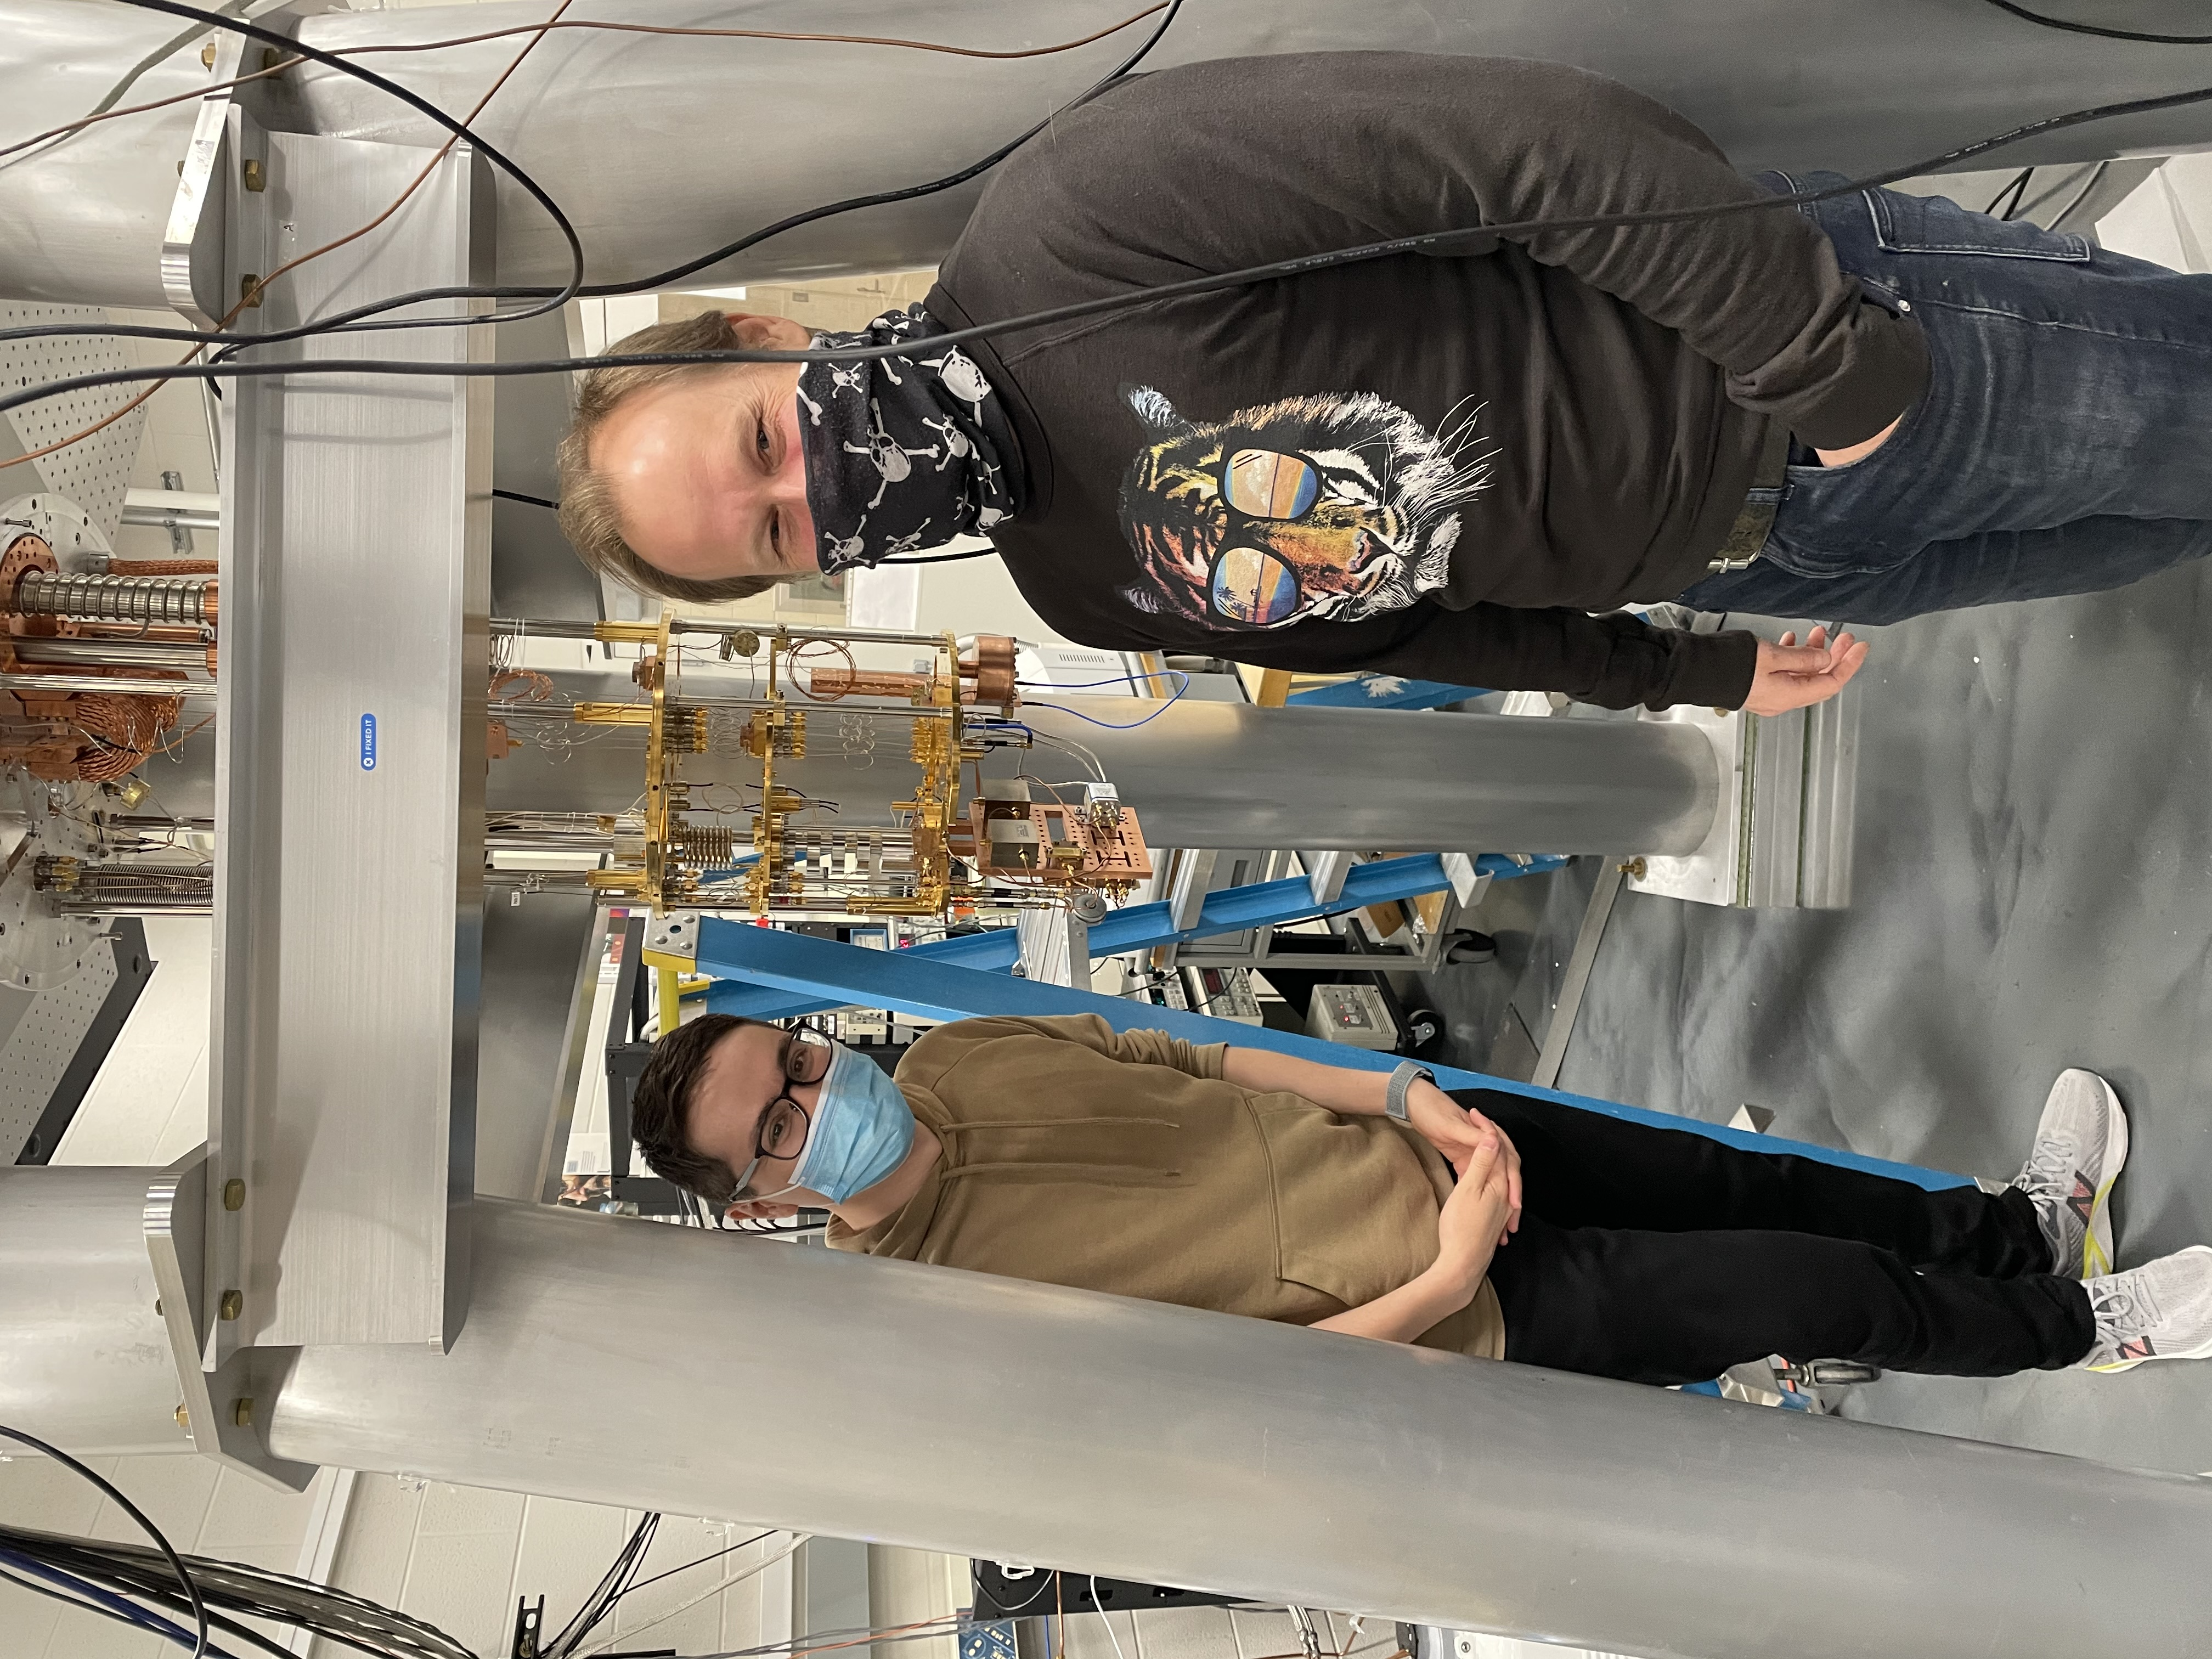
\includegraphics[width=1.3\textwidth]{qcfigures/lab.jpeg}}
      \end{center}
\end{columns}
      \end{footnotesize}
    }




\frame
    {
      \frametitle{Single electrons can make great qubits}
	
      \begin{footnotesize}
     \begin{columns}
       \column{5.0cm}

       At the heart is the trapping and control
       of individual electrons floating above pools of superfluid
       helium. These electrons form the qubits of our quantum
       computer, and the purity of the superfluid helium protects the
       intrinsic quantum properties of each electron. The  ultimate
       goal is to build a large-scale quantum computer based on
       quantum magnetic (spin) state of these trapped electrons.
\column{5cm}
      \begin{center}
	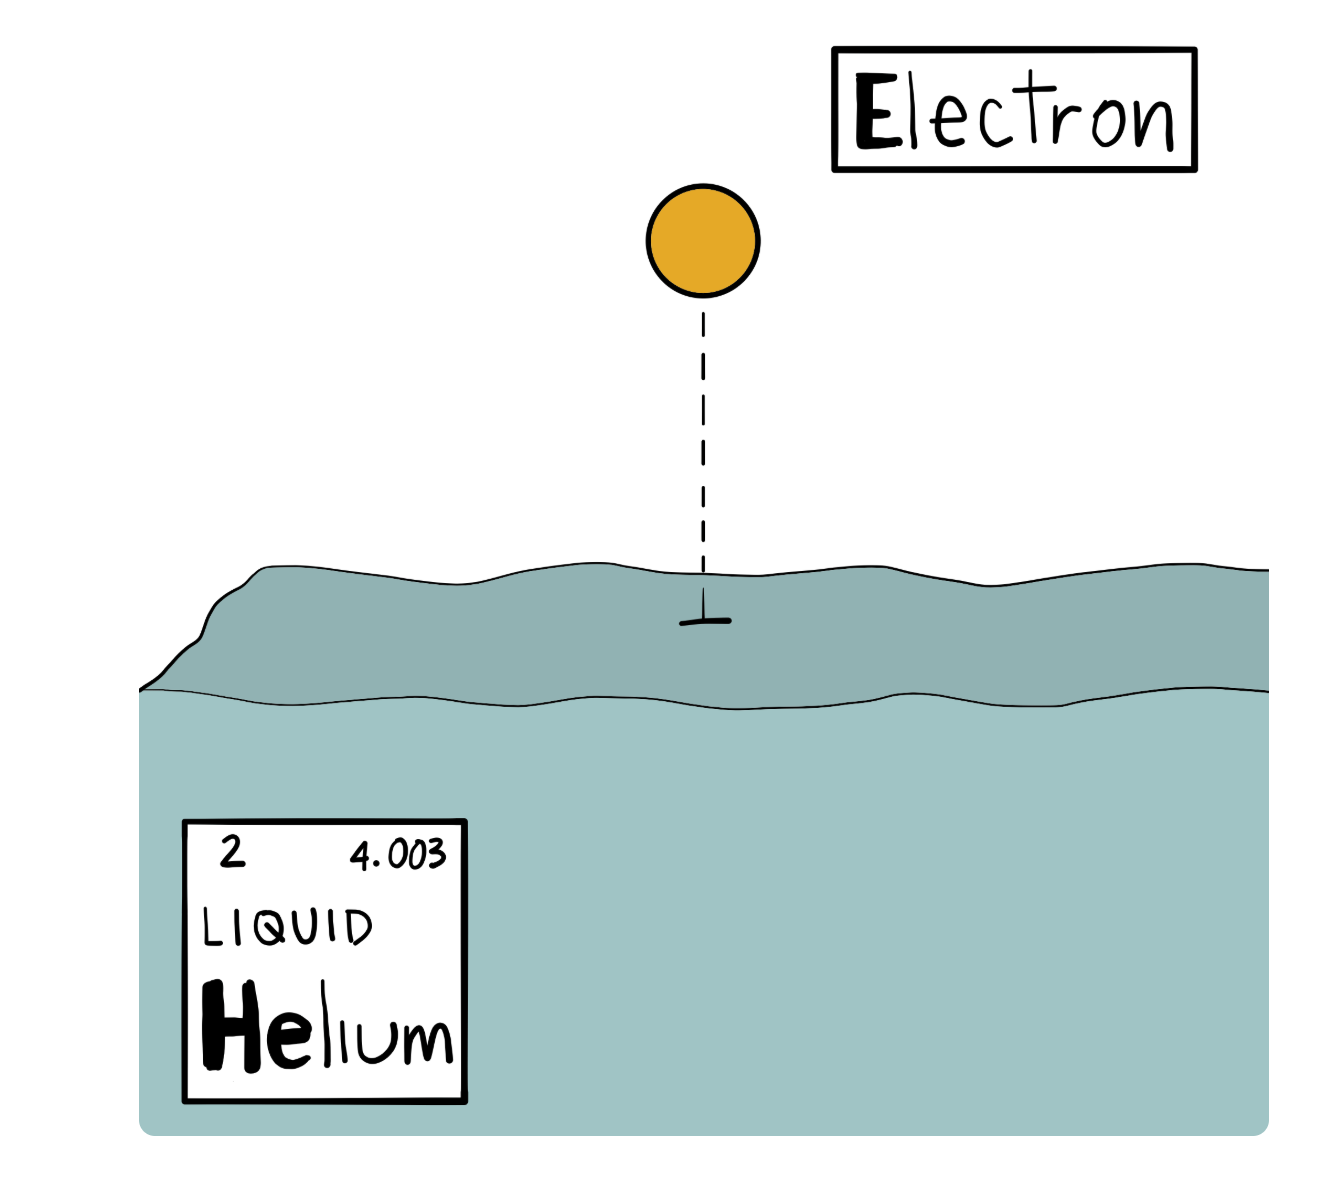
\includegraphics[width=1.2\textwidth]{qcfigures/nordicquantumfig1.png}
      \end{center}
\end{columns}
      \end{footnotesize}
    }


\frame
    {
      \frametitle{Trapping electrons in microchannels}
	
      \begin{footnotesize}
     \begin{columns}
       \column{5.0cm}
Microchannels fabricated into silicon wafers are filled with superfluid helium and energized electrodes. Together with the natural electron trapping properties of superfluid helium, these allow for the precision trapping of individual or multiple electrons. The microchannels are only a few micrometers in size, or about five times smaller than the diameter of a human hair.
\column{5cm}
      \begin{center}
	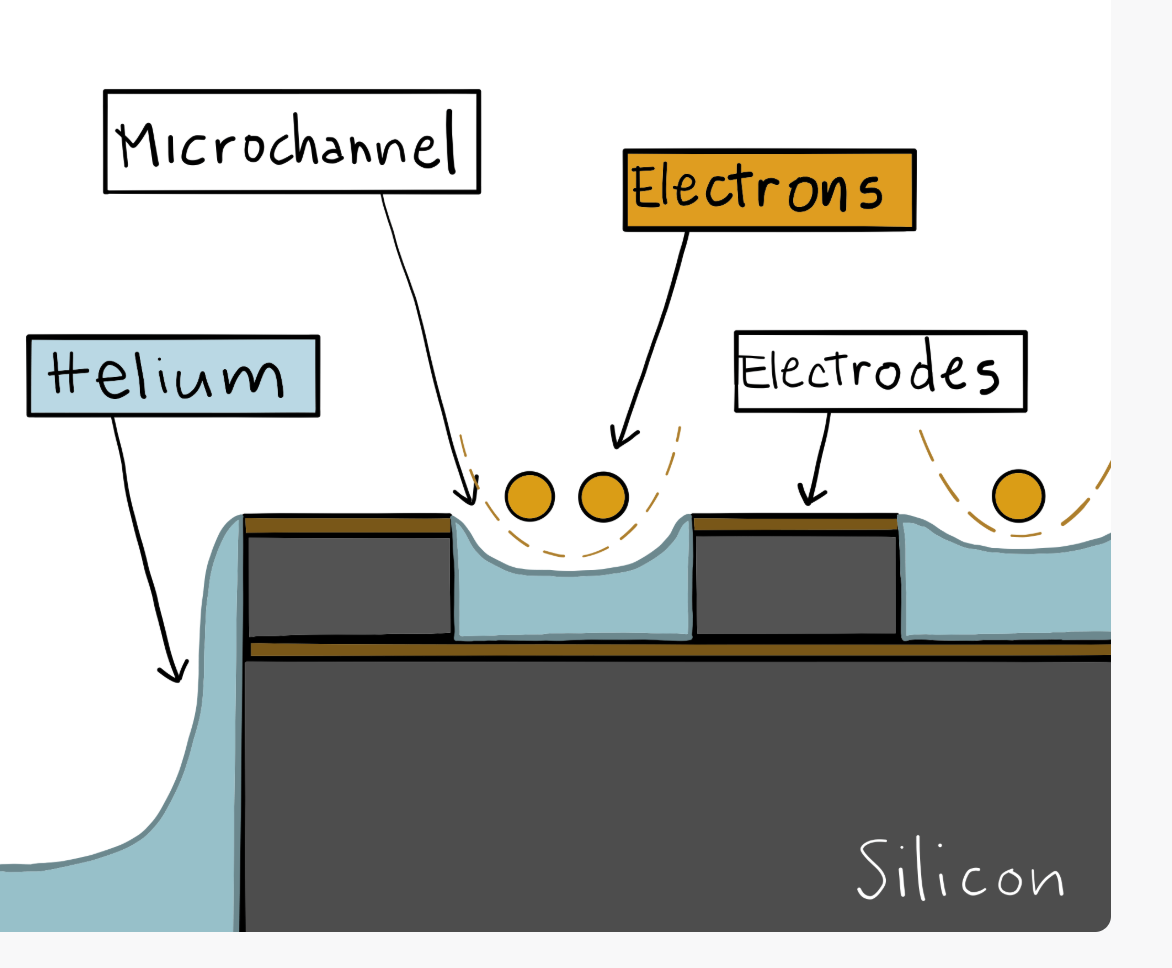
\includegraphics[width=1.2\textwidth]{qcfigures/nordicquantumfig2.png}
      \end{center}
\end{columns}
      \end{footnotesize}
    }

\frame
    {
      \frametitle{Control and readout}
	
      \begin{footnotesize}
     \begin{columns}
       \column{5.0cm}

       Microchannel regions can store thousands of electrons, from which one can be plucked and transported to the single electron control and readout area. In this region, microwave signals will interact with the electron to perform quantum logic gate operations, which will be readout via extremely fast electronics.


\column{5cm}
      \begin{center}
	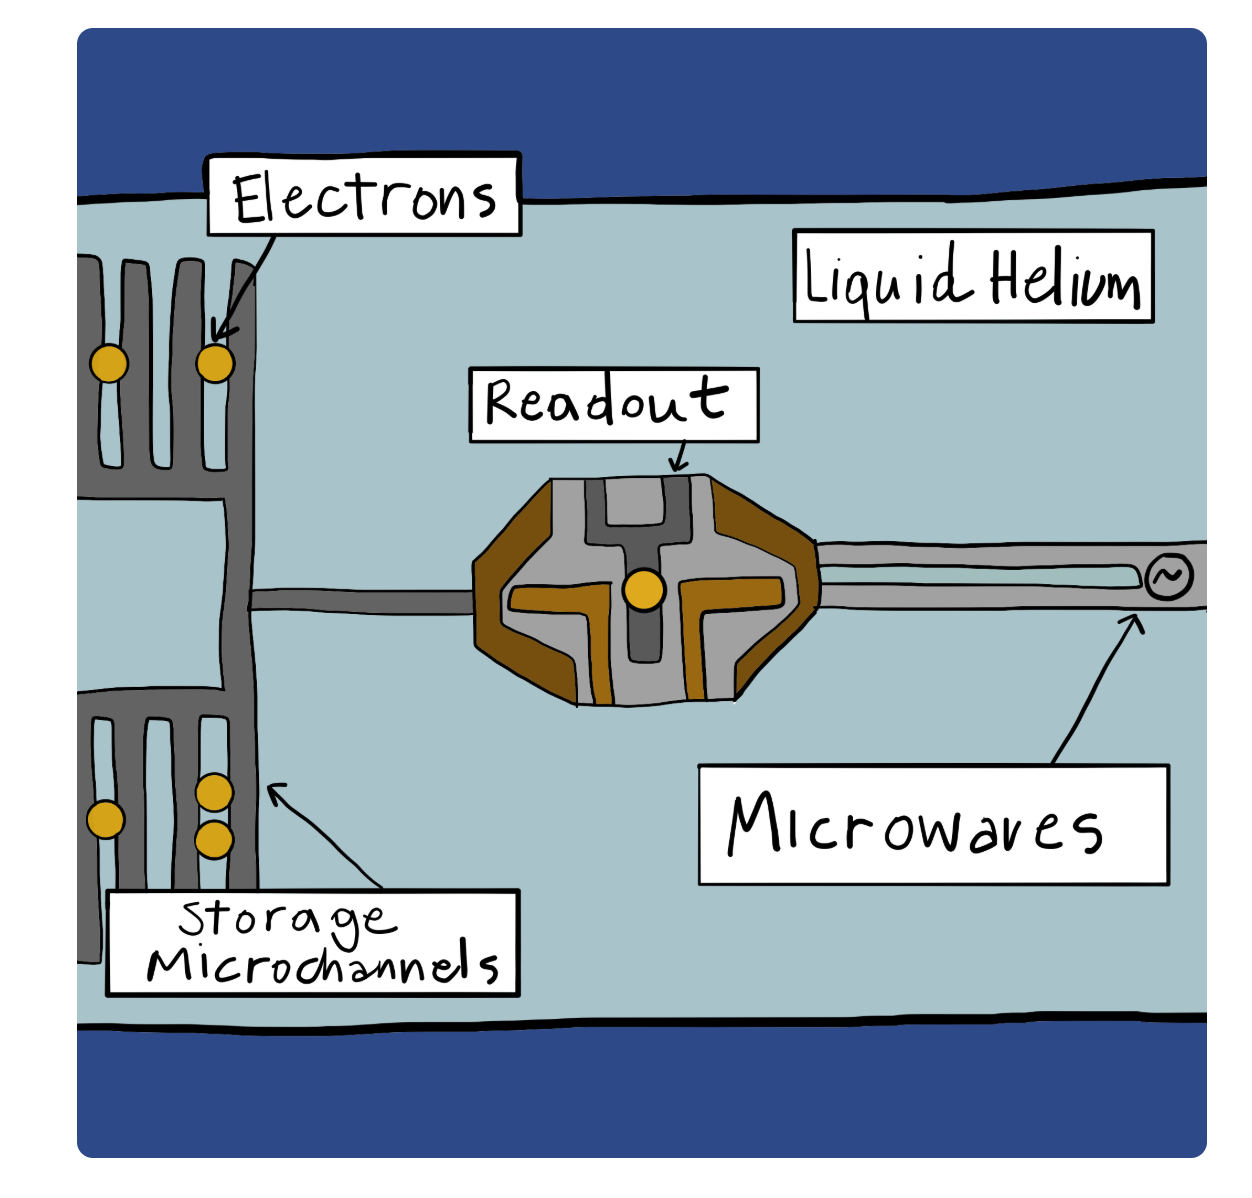
\includegraphics[width=1.2\textwidth]{qcfigures/nordicquantumfig3.png}
      \end{center}
\end{columns}
      \end{footnotesize}
    }


\frame
    {
      \frametitle{Operations for quantum computing}
	
      \begin{footnotesize}
     \begin{columns}
       \column{5.0cm}
Quantum information can be encoded in a number of ways using single electrons. Currently, we are working with the side-to-side(lateral) quantum motion of the electron in the engineered trap. This motion can either be in its lowest energy state, the ground state, or in a number of higher-energy excited states. This electron motion also provides the readout capabilities for the ultimate goal of building a large-scale quantum computer based on the electron's magnetic moment (spin).       
\column{5cm}
      \begin{center}
	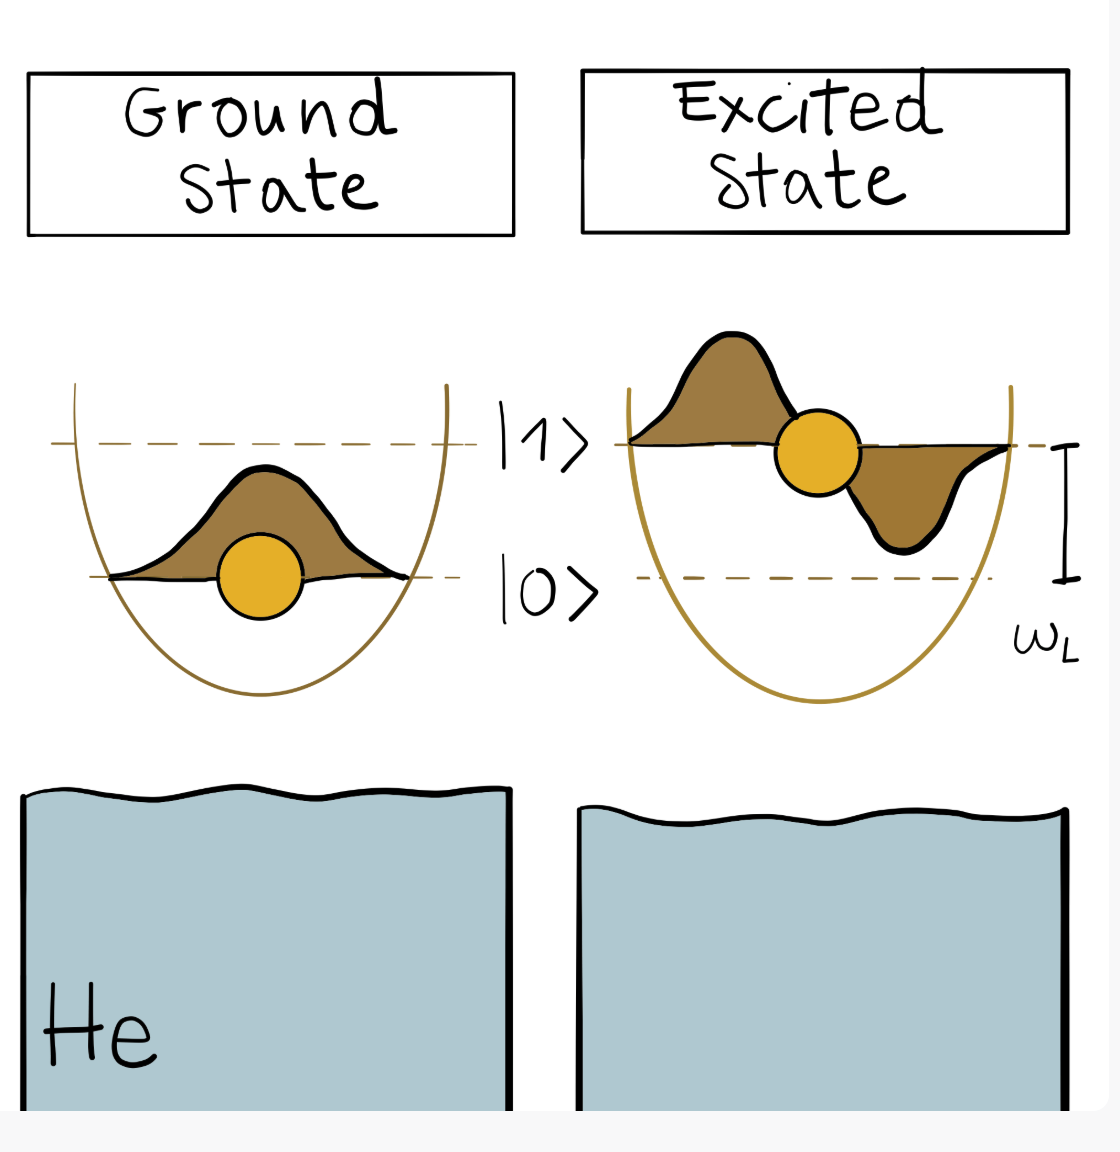
\includegraphics[width=1.2\textwidth]{qcfigures/nordicquantumfig4.png}
      \end{center}
\end{columns}
      \end{footnotesize}
    }


\end{document}
